

% \newcommand{\examplecommon}[3]{
% \begin{figure}[b]
% \begin{center}
% \hspace*{-0.98\textwidth}
% \includegraphics[width=0.19\textwidth,keepaspectratio,bb=0 0 100 100]{chapters/Algorithms/examples/#1.pdf}
% \caption{#2}
% {#3}
% \end{center}
% \end{figure}
% }

% \newcommand{\exampleStep}[1]{
% \begin{figure}[b]
% \begin{center}
% \hspace*{-0.98\textwidth}
% \includegraphics[width=0.19\textwidth,keepaspectratio,bb=0 0 100 100]{chapters/Algorithms/examples/ca/#1.pdf}
% % \caption{#2}
% % {#3}
% \end{center}
% \end{figure}
% }

\newcommand{\examplecommon}[3]{

\begin{figure}[h]
\begin{center}
\hspace*{-0.1\textwidth}
\includegraphics[width=1.1\textwidth]{chapters/Algorithms/examples/all/#1.pdf}
\vspace{-20pt}
\caption{#2}
{#3}
\end{center}
\end{figure}
}

\newcommand{\exampleStep}[4]{
\begin{figure}[h]
\begin{center}
\hspace*{-0.1\textwidth}
\includegraphics[width=1.1\textwidth]{chapters/Algorithms/examples/#1/#1#2.pdf}
\caption{}
{#3}
\end{center}
\end{figure}
}


% \newcommand{\examplelinear}{
% \begin{figure}[h]
% \begin{center}
% \hspace*{-0.1\textwidth}
% \includegraphics[width=0.6\textwidth]{chapters/Algorithms/examples/all/linear.pdf}
% \vspace{-10pt}
% \caption{Example Linear}
% \label{example:linear}
% \end{center}
% \end{figure}
% }

\newcommand{\examplelinear}{
\centering
\includegraphics[width=1.2\textwidth]{chapters/Algorithms/examples/linear.pdf}
\vspace{-5pt}
\begin{minipage}{1.17\textwidth}
\captionof{figure}{Example of the auxiliary routine \decodeSegment\ for linear model algorithms.}
\label{example:linear}
\end{minipage}
}

\newcommand{\examplePWLH}{
\begin{figure}[h]
% \centering
\hspace{-30pt}
\begin{minipage}{.55\textwidth}
  \centering
  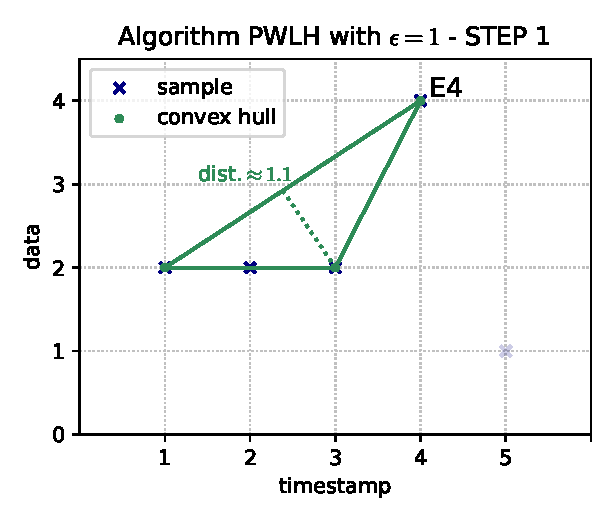
\includegraphics[width=1.0\linewidth]{chapters/Algorithms/examples/pwlh_intro/pwlh1.pdf}
  \captionof{figure}{}
  \label{example:pwlhIntro1}
\end{minipage}%
\begin{minipage}{.55\textwidth}
  \centering
  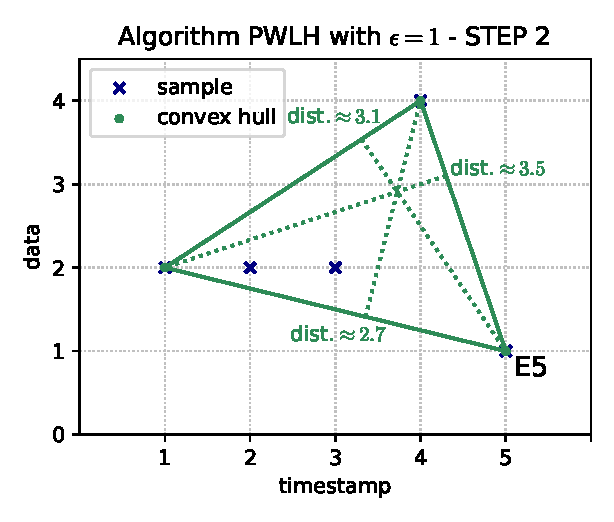
\includegraphics[width=1.0\linewidth]{chapters/Algorithms/examples/pwlh_intro/pwlh2.pdf}
  \captionof{figure}{}
  \label{example:pwlhIntro2}
\end{minipage}
\end{figure}
}

\newcommand{\exampleCA}{
\begin{figure}[h]
% \centering
\hspace{-30pt}
\begin{minipage}{.55\textwidth}
  \centering
  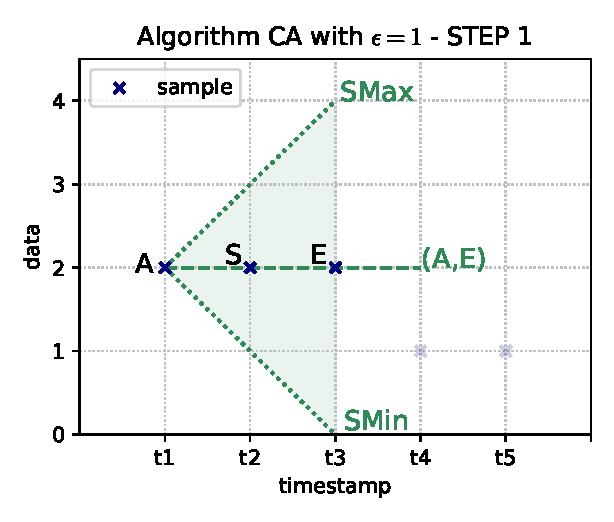
\includegraphics[width=1.0\linewidth]{chapters/Algorithms/examples/ca_intro/ca1.pdf}
  \captionof{figure}{}
  \label{example:caIntro1}
\end{minipage}%
\begin{minipage}{.55\textwidth}
  \centering
  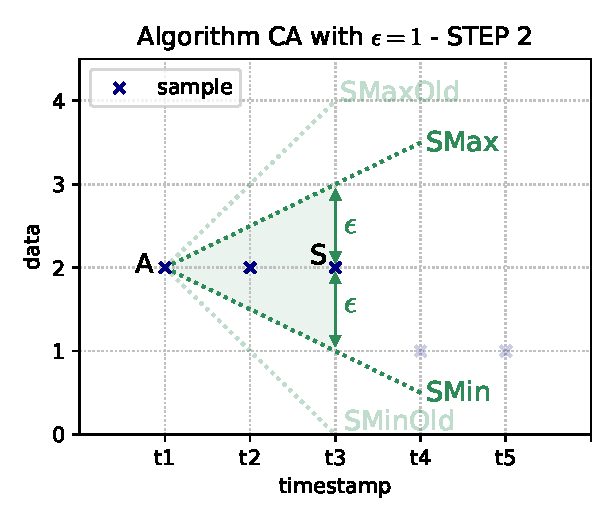
\includegraphics[width=1.0\linewidth]{chapters/Algorithms/examples/ca_intro/ca2.pdf}
  \captionof{figure}{}
  \label{example:caIntro2}
\end{minipage}
\end{figure}
}

\newcommand{\exampleSF}{
\begin{figure}[h]
% \centering
\hspace{-30pt}
\begin{minipage}{.55\textwidth}
  \centering
  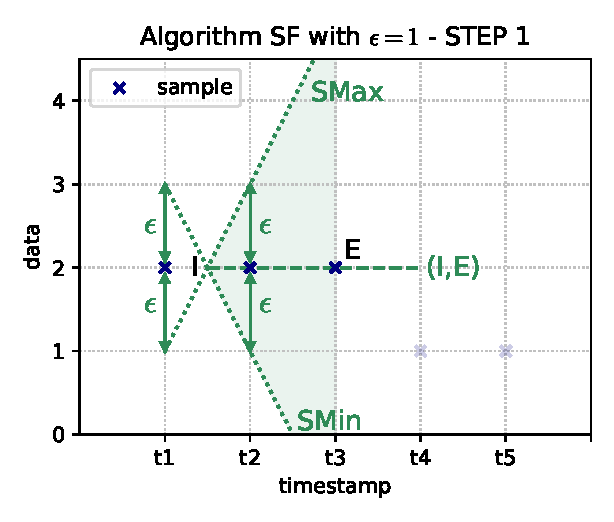
\includegraphics[width=1.0\linewidth]{chapters/Algorithms/examples/sf_intro/sf1.pdf}
  \captionof{figure}{}
  \label{example:sfIntro1}
\end{minipage}%
\begin{minipage}{.55\textwidth}
  \centering
  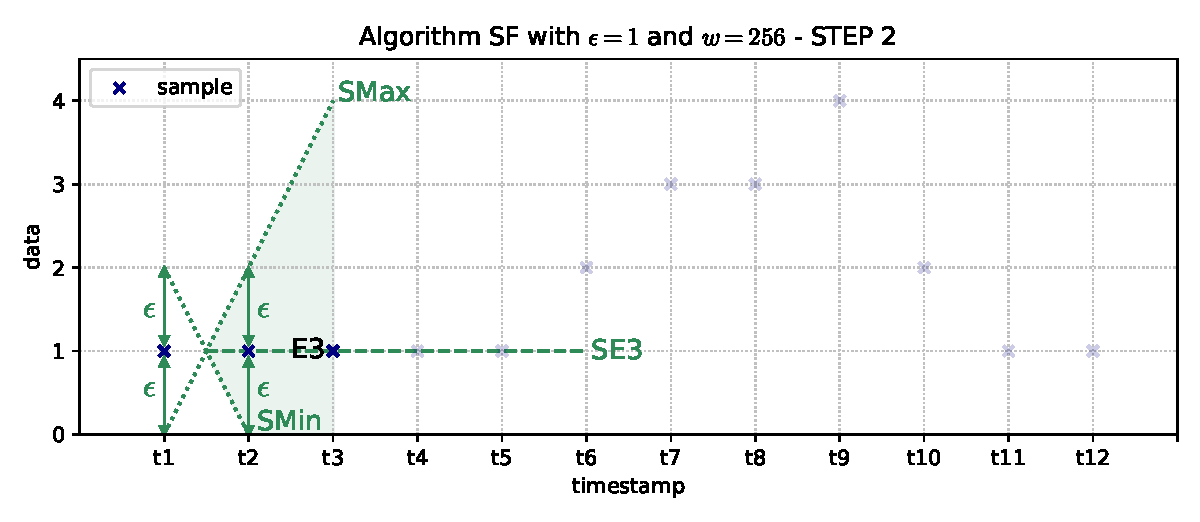
\includegraphics[width=1.0\linewidth]{chapters/Algorithms/examples/sf_intro/sf2.pdf}
  \captionof{figure}{}
  \label{example:sfIntro2}
\end{minipage}
\end{figure}
}
